\documentclass[11pt,a4paper]{article}

%------------------------------------------------
% IDIOMA Y CODIFICACIÓN
%------------------------------------------------
\usepackage[spanish]{babel}
\usepackage[utf8]{inputenc}
\usepackage[T1]{fontenc}

%------------------------------------------------
% PAQUETES
%------------------------------------------------
\usepackage{graphicx}
\usepackage{eso-pic}
\usepackage{xcolor}
\usepackage{geometry}
\geometry{margin=2cm}
\pagestyle{empty}

\usepackage{titlesec}
\usepackage{parskip}
\usepackage{tcolorbox}
\usepackage{hyperref}
\usepackage{fontawesome5}
\usepackage{amssymb}

\usepackage{mathpazo}

%========================
% COLORES
%========================

\definecolor{ForestGreen}{HTML}{355E3B}
\definecolor{SoftGreen}{HTML}{7BA05B}
\definecolor{Stone}{HTML}{E8E5DF}
\definecolor{Beige}{HTML}{F7F3EA}
\definecolor{Brown}{HTML}{4B3F35}

\begin{document}

%%%%%%%%%%%%%%%%%%%%%%%%%%%%%%%%%%%%%%%%%%
% PORTADA
%%%%%%%%%%%%%%%%%%%%%%%%%%%%%%%%%%%%%%%%%%

\newgeometry{
left=0cm,
right=0cm,
top=0cm,
bottom=0cm
}

\AddToShipoutPictureBG*{%
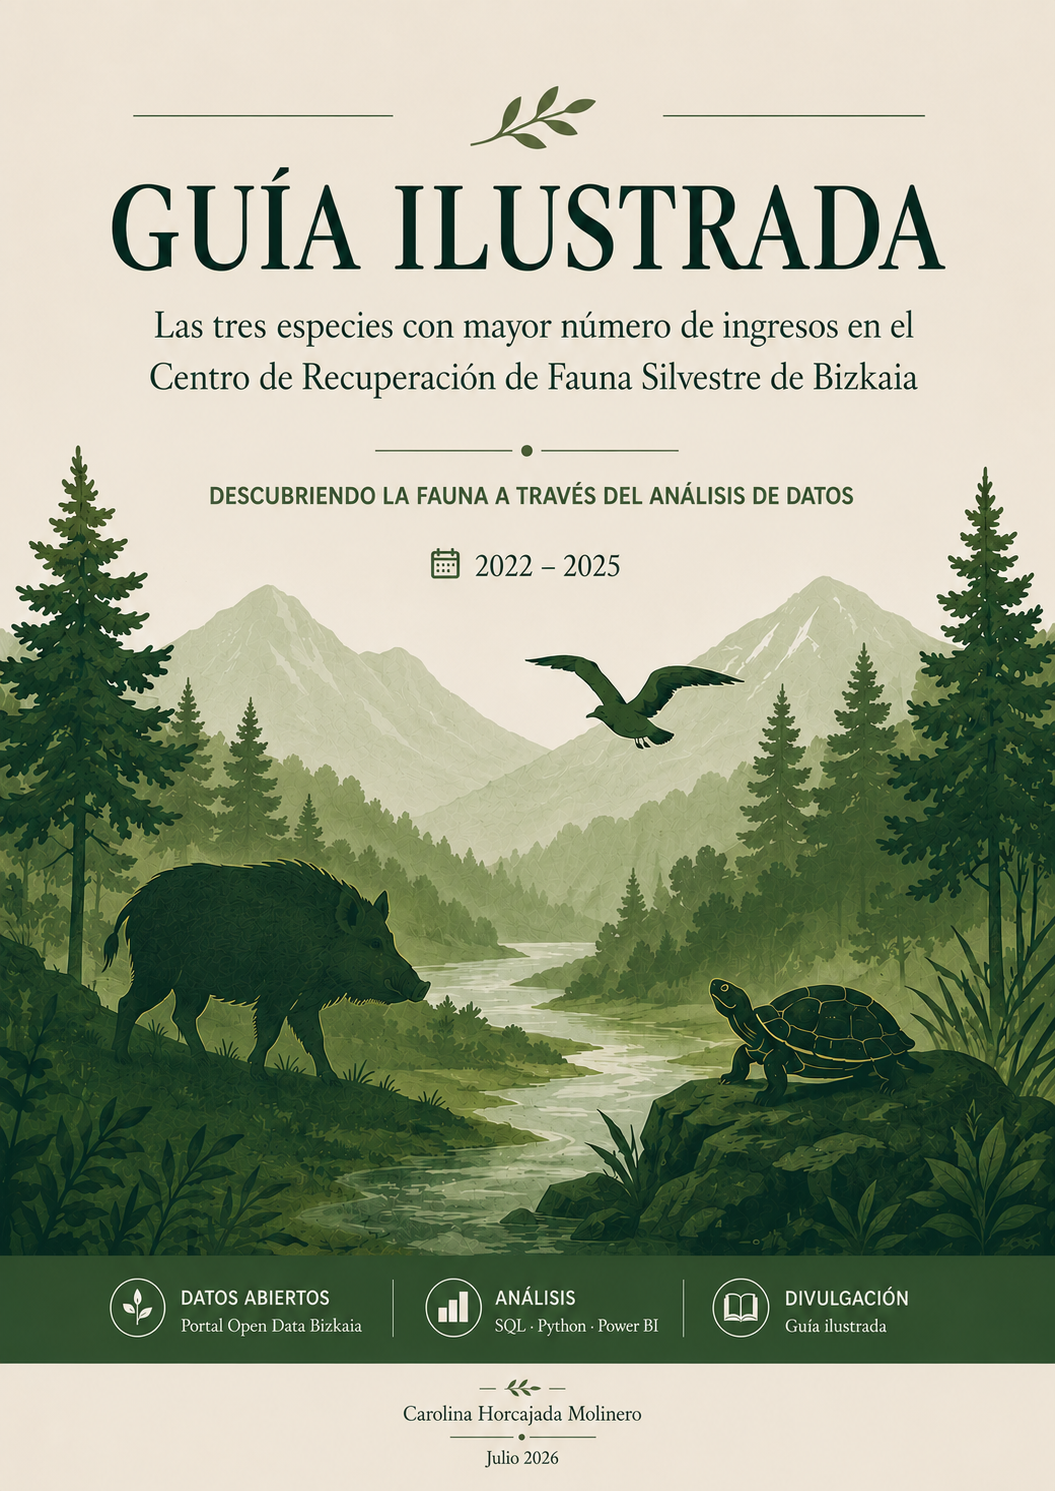
\includegraphics[
width=\paperwidth,
height=\paperheight
]{images/guia_portada.png}
}

\mbox{}

\ClearShipoutPictureBG

\restoregeometry

\clearpage


%%%%%%%%%%%%%%%%%%%%%%%%%%%%%%%%%%%%%%%%%%
% PÁGINA 2
%%%%%%%%%%%%%%%%%%%%%%%%%%%%%%%%%%%%%%%%%%

%%%%%%%%%%%%%%%%%%%%%%%%%%%%%%%%%%%%%%%%%%
% ¿QUÉ ES ESTA GUÍA?
%%%%%%%%%%%%%%%%%%%%%%%%%%%%%%%%%%%%%%%%%%

\thispagestyle{empty}

{\color{SoftGreen}\rule{\textwidth}{1pt}}

\vspace{0.6cm}

\begin{center}

{\fontsize{24}{28}\selectfont
\textcolor{ForestGreen}{\textbf{¿QUÉ ES ESTA GUÍA?}}
}

\end{center}

\vspace{0.5cm}

\begin{center}
\begin{minipage}{0.86\textwidth}

{\large

\faLeaf\ Esta guía nace como complemento del dashboard desarrollado en Power BI y transforma datos abiertos en una publicación divulgativa sobre la fauna atendida en el Centro de Recuperación de Fauna Silvestre de Bizkaia.

\vspace{0.35cm}

\faDatabase\ Los datos proceden del Portal de Datos Abiertos de la Diputación Foral de Bizkaia e incluyen todos los ingresos registrados entre los años 2022 y 2025.

\vspace{0.35cm}

\faBroom\ Antes del análisis fue necesario realizar un proceso completo de limpieza, transformación y preparación de los datos.

\vspace{0.35cm}

\faChartBar\ Finalmente, la información fue analizada mediante Python y Power BI para identificar patrones, tendencias y especies con mayor frecuencia de ingreso.

}

\end{minipage}
\end{center}

\vspace{0.7cm}

%%%%%%%%%%%%%%%%%%%%%%%%%%%%%%%%%%%%%%%%%%%%%%
% ESQUEMA
%%%%%%%%%%%%%%%%%%%%%%%%%%%%%%%%%%%%%%%%%%%%%%

\begin{tcolorbox}[
colback=Beige,
colframe=ForestGreen,
arc=4mm,
title=\textbf{\faProjectDiagram\ Del dato a la guía},
fonttitle=\bfseries]

\begin{center}

\Large

Datos abiertos

$\downarrow$

Limpieza y preparación

$\downarrow$

Python

$\downarrow$

Dashboard Power BI

$\downarrow$

Guía ilustrada

\end{center}

\end{tcolorbox}

\vspace{0.45cm}

\begin{center}

\small

Cada una de las especies presentadas en esta guía ha sido seleccionada a partir del análisis de los registros con mayor número de ingresos en el Centro de Recuperación de Fauna Silvestre de Bizkaia entre 2022 y 2025.

\end{center}

\vspace{0.35cm}

%%%%%%%%%%%%%%%%%%%%%%%%%%%%%%%%%%%%%%%%%%%%%%
% OBJETIVO
%%%%%%%%%%%%%%%%%%%%%%%%%%%%%%%%%%%%%%%%%%%%%%

\begin{tcolorbox}[
colback=Stone,
colframe=SoftGreen,
arc=3mm,
title=\textbf{\faLightbulb\ Objetivo del proyecto},
fonttitle=\bfseries]

Mostrar cómo el análisis de datos puede convertirse en una herramienta divulgativa capaz de acercar la biodiversidad al público general mediante visualizaciones y fichas ilustradas de las especies con mayor número de ingresos.

\end{tcolorbox}

\vfill

\begin{center}

\small

\faCalendar\ 2022--2025
\hspace{1.8cm}
\faPaw\ Top 3 especies
\hspace{1.8cm}
\faChartBar\ Dashboard interactivo

\vspace{0.35cm}

\end{center}

%%%%%%%%%%%%%%%%%%%%%%%%%%%%%%%%%%%%%%%%%%%%%%%%%%%%%%%%%%%%
% PAGINA 3
% JABALI
%%%%%%%%%%%%%%%%%%%%%%%%%%%%%%%%%%%%%%%%%%%%%%%%%%%%%%%%%%%%

\newpage
\thispagestyle{empty}

\begin{center}

{\fontsize{24}{28}\selectfont
\textcolor{ForestGreen}{\textbf{JABALÍ}}
}

\vspace{0.1cm}

{\large\itshape Sus scrofa}

\vspace{0.15cm}

{\color{SoftGreen}\rule{0.28\textwidth}{0.5pt}}

\vspace{0.45cm}

\vspace{0.8cm}

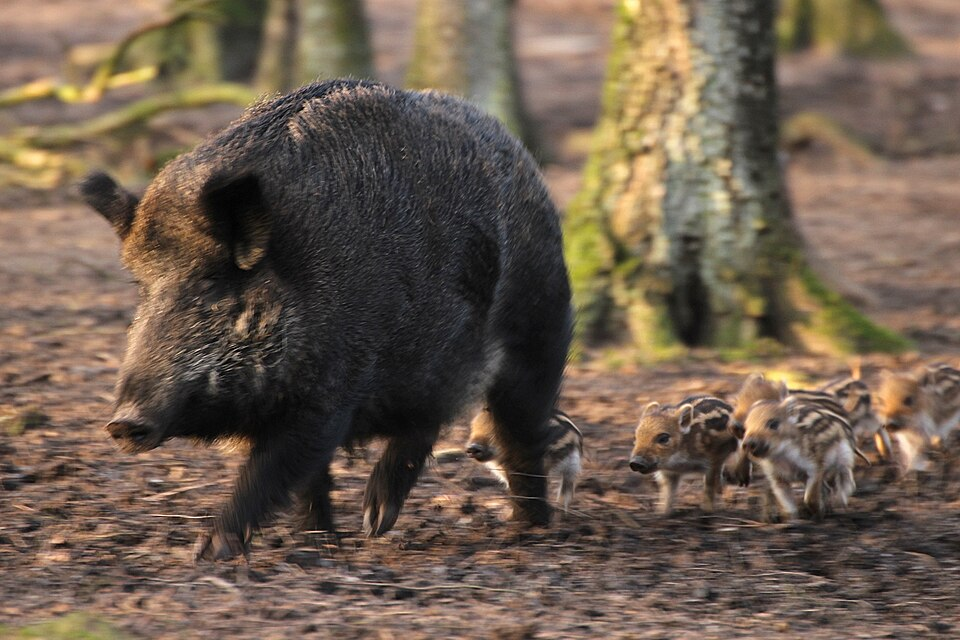
\includegraphics[width=0.82\textwidth,height=8cm,keepaspectratio]{images/jabali.jpg}

\end{center}

\begin{center}

\large\itshape
"La especie de mamífero con mayor número de ingresos
registrados en el estudio."

\end{center}

\vspace{0.5cm}

%%%%%%%%%%%%%%%%%%%%%%%%%%%%%%%%%%%%%%
% DESCRIPCION
%%%%%%%%%%%%%%%%%%%%%%%%%%%%%%%%%%%%%%

{\Large\textcolor{Brown}{\textbf{Descripción}}}

\vspace{0.2cm}

\begin{quote}

El jabalí fue la segunda especie con mayor número de ingresos
registrados durante el periodo analizado (2022--2025).

Su elevada presencia está relacionada con el aumento de la interacción
entre la fauna silvestre y las actividades humanas, especialmente
en áreas periurbanas y carreteras.

\end{quote}

\vspace{0.45cm}

%%%%%%%%%%%%%%%%%%%%%%%%%%%%%%%%%%%%%%
% RESULTADOS
%%%%%%%%%%%%%%%%%%%%%%%%%%%%%%%%%%%%%%

\begin{tcolorbox}[
colback=Beige,
colframe=ForestGreen,
title=\faChartBar\ Resultados del análisis,
fonttitle=\bfseries]

\begin{tabular}{ll}

\textbf{Ingresos registrados} & 383 \\

\textbf{Posición} & 2ª especie con más ingresos \\

\textbf{Clase} & Mamíferos \\

\textbf{Periodo} & 2022--2025 \\

\end{tabular}

\end{tcolorbox}

\vspace{0.25cm}

%%%%%%%%%%%%%%%%%%%%%%%%%%%%%%%%%%%%%%
% CURIOSIDAD
%%%%%%%%%%%%%%%%%%%%%%%%%%%%%%%%%%%%%%

\begin{tcolorbox}[
colback=Stone,
colframe=SoftGreen,
title=\faLightbulb\ ¿Sabías que...?,
fonttitle=\bfseries]

Los jabalíes pueden recorrer más de 10 kilómetros en una sola noche.

Su extraordinario olfato les permite localizar alimento incluso bajo
varios centímetros de tierra.

\end{tcolorbox}

\vspace{0.25cm}

%%%%%%%%%%%%%%%%%%%%%%%%%%%%%%%%%%%%%%
% PEGATINA
%%%%%%%%%%%%%%%%%%%%%%%%%%%%%%%%%%%%%%

\begin{flushright}

\fcolorbox{Brown}{Beige}{

\begin{minipage}{0.34\textwidth}
\centering

\large
\faExclamationTriangle\ ¡No me alimentes!

\small

Después volveré con
toda mi familia...

\end{minipage}

}

\end{flushright}

%%%%%%%%%%%%%%%%%%%%%%%%%%%%%%%%%%%%%%%%%%%%%%%%%%%%%%%%%%%%
% PAGINA 4
% GAVIOTA PATIAMARILLA
%%%%%%%%%%%%%%%%%%%%%%%%%%%%%%%%%%%%%%%%%%%%%%%%%%%%%%%%%%%%

\newpage
\thispagestyle{empty}

\begin{center}

{\fontsize{24}{28}\selectfont
\textcolor{ForestGreen}{\textbf{GAVIOTA PATIAMARILLA}}
}

\vspace{0.1cm}

{\large\itshape Larus michahellis}

\vspace{0.15cm}

{\color{SoftGreen}\rule{0.28\textwidth}{0.5pt}}

\vspace{0.45cm}

\vspace{0.8cm}

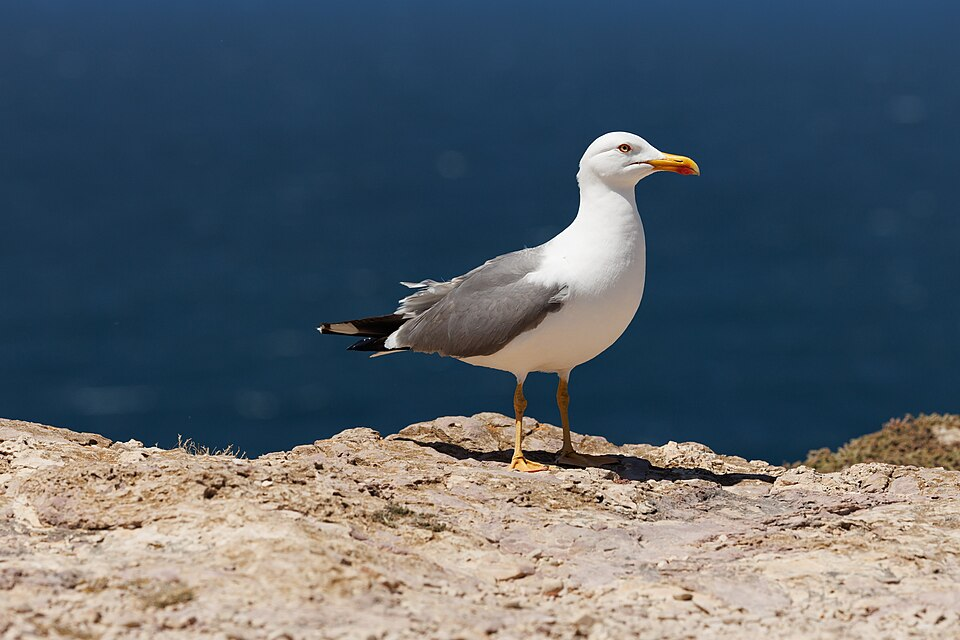
\includegraphics[width=0.82\textwidth,height=8cm,keepaspectratio]{images/gaviota.jpg}

\end{center}

\begin{center}

\large\itshape
"La especie con mayor número de ingresos
registrados entre 2022 y 2025."

\end{center}

\vspace{0.5cm}

%%%%%%%%%%%%%%%%%%%%%%%%%%%%%%%%%%%%%%
% DESCRIPCIÓN
%%%%%%%%%%%%%%%%%%%%%%%%%%%%%%%%%%%%%%

{\Large\textcolor{Brown}{\textbf{Descripción}}}

\vspace{0.2cm}

\begin{quote}

Con \textbf{445 ingresos registrados entre 2022 y 2025},
la gaviota patiamarilla fue la especie con mayor presencia
en el Centro de Recuperación de Fauna Silvestre de Bizkaia.

Su abundancia y su estrecha convivencia con las personas
hacen que sea una de las especies que con mayor frecuencia
requiere atención por traumatismos, pollos caídos del nido
o situaciones derivadas de la actividad humana.

\end{quote}

\vspace{0.45cm}

%%%%%%%%%%%%%%%%%%%%%%%%%%%%%%%%%%%%%%
% RESULTADOS
%%%%%%%%%%%%%%%%%%%%%%%%%%%%%%%%%%%%%%

\begin{tcolorbox}[
colback=Beige,
colframe=ForestGreen,
title=\faChartBar\ Resultados del análisis,
fonttitle=\bfseries]

\begin{tabular}{ll}

\textbf{Ingresos registrados} & 445 \\

\textbf{Posición} & 1ª especie con más ingresos \\

\textbf{Clase} & Aves \\

\textbf{Periodo} & 2022--2025 \\

\end{tabular}

\end{tcolorbox}

\vspace{0.25cm}

%%%%%%%%%%%%%%%%%%%%%%%%%%%%%%%%%%%%%%
% CURIOSIDAD
%%%%%%%%%%%%%%%%%%%%%%%%%%%%%%%%%%%%%%

\begin{tcolorbox}[
colback=Stone,
colframe=SoftGreen,
title=\faLightbulb\ ¿Sabías que...?,
fonttitle=\bfseries]

Las gaviotas son capaces de reconocer rostros humanos y
recordar durante años a las personas que consideran una
amenaza o una fuente habitual de alimento.

\end{tcolorbox}

\vspace{0.25cm}

%%%%%%%%%%%%%%%%%%%%%%%%%%%%%%%%%%%%%%
% PEGATINA
%%%%%%%%%%%%%%%%%%%%%%%%%%%%%%%%%%%%%%

\begin{flushright}

\fcolorbox{Brown}{Beige}{

\begin{minipage}{0.34\textwidth}
\centering

\large
\faUtensils\ ¡No me des comida!

\small

Alimentarme altera
mi comportamiento.

\end{minipage}

}

\end{flushright}

%%%%%%%%%%%%%%%%%%%%%%%%%%%%%%%%%%%%%%%%%%%%%%%%%%%%%%%%%%%%
% PAGINA 5
% TORTUGA DE FLORIDA
%%%%%%%%%%%%%%%%%%%%%%%%%%%%%%%%%%%%%%%%%%%%%%%%%%%%%%%%%%%%

\newpage
\thispagestyle{empty}

\begin{center}

{\fontsize{24}{28}\selectfont
\textcolor{ForestGreen}{\textbf{TORTUGA DE OREJAS AMARILLAS}}
}

\vspace{0.1cm}

{\large\itshape Trachemys scripta scripta}

\vspace{0.15cm}

{\color{SoftGreen}\rule{0.28\textwidth}{0.5pt}}

\vspace{0.45cm}

\vspace{0.8cm}

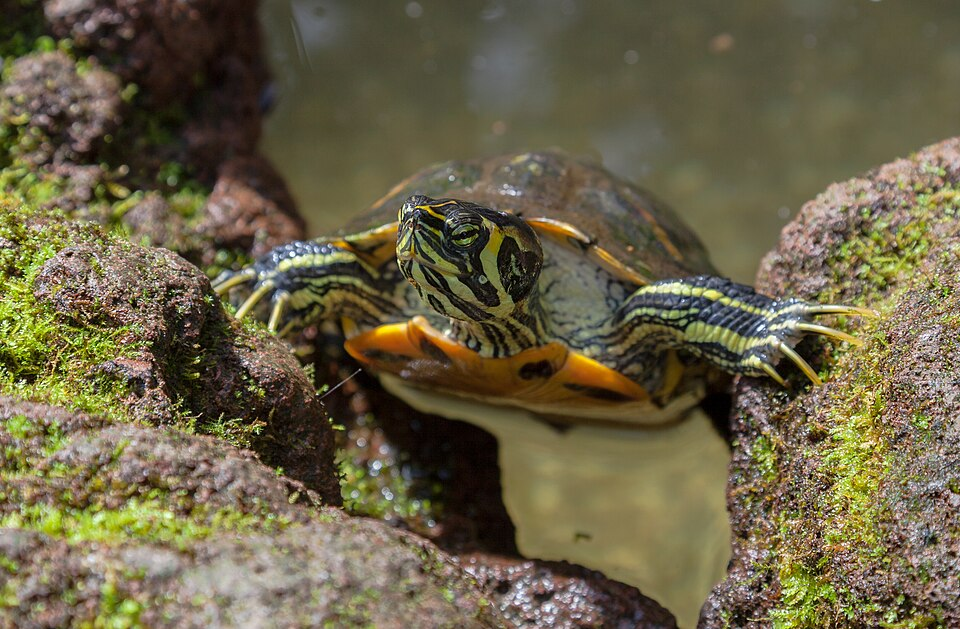
\includegraphics[width=0.82\textwidth,height=8cm,keepaspectratio]{images/tortuga.jpg}

\end{center}

\begin{center}

{\large\itshape
``El reptil con mayor número de ingresos
registrados en el estudio.''
}

\end{center}

\vspace{0.5cm}

%%%%%%%%%%%%%%%%%%%%%%%%%%%%%%%%%%%%%%
% DESCRIPCIÓN
%%%%%%%%%%%%%%%%%%%%%%%%%%%%%%%%%%%%%%

{\Large\textcolor{Brown}{\textbf{Descripción}}}

\vspace{0.2cm}

\begin{quote}

La tortuga de Florida de Orejas Amarillas registró \textbf{379 ingresos}
durante el periodo 2022--2025, convirtiéndose en el reptil
más frecuente del Centro de Recuperación de Fauna Silvestre
de Bizkaia.

Se trata de una especie exótica invasora cuya presencia
en el medio natural supone una amenaza para las tortugas
autóctonas y otros ecosistemas acuáticos.

\end{quote}

\vspace{0.45cm}

%%%%%%%%%%%%%%%%%%%%%%%%%%%%%%%%%%%%%%
% RESULTADOS
%%%%%%%%%%%%%%%%%%%%%%%%%%%%%%%%%%%%%%

\begin{tcolorbox}[
colback=Beige,
colframe=ForestGreen,
title=\faChartBar\ Resultados del análisis,
fonttitle=\bfseries]

\begin{tabular}{ll}

\textbf{Ingresos registrados} & 379 \\

\textbf{Posición} & 3ª especie con más ingresos \\

\textbf{Clase} & Reptiles \\

\textbf{Periodo} & 2022--2025 \\

\end{tabular}

\end{tcolorbox}

\vspace{0.25cm}

%%%%%%%%%%%%%%%%%%%%%%%%%%%%%%%%%%%%%%
% CURIOSIDAD
%%%%%%%%%%%%%%%%%%%%%%%%%%%%%%%%%%%%%%

\begin{tcolorbox}[
colback=Stone,
colframe=SoftGreen,
title=\faLightbulb\ ¿Sabías que...?,
fonttitle=\bfseries]

La tortuga de Florida puede vivir más de 30 años.
Muchas fueron compradas como mascota y posteriormente
liberadas, lo que ha favorecido su expansión por
humedales de toda Europa.

\end{tcolorbox}

\vspace{0.25cm}

%%%%%%%%%%%%%%%%%%%%%%%%%%%%%%%%%%%%%%
% PEGATINA
%%%%%%%%%%%%%%%%%%%%%%%%%%%%%%%%%%%%%%

\begin{flushright}

\fcolorbox{Brown}{Beige}{

\begin{minipage}{0.34\textwidth}
\centering

\large
\faPaw\ No me abandones

\small

Liberarme en la naturaleza
daña el ecosistema.

\end{minipage}

}

\end{flushright}


%%%%%%%%%%%%%%%%%%%%%%%%%%%%%%%%%%%%%%%%%%%%%%%%%%%%%%%%%%%%
% PAGINA 6
% CONCLUSIONES
%%%%%%%%%%%%%%%%%%%%%%%%%%%%%%%%%%%%%%%%%%%%%%%%%%%%%%%%%%%%

\newpage
\thispagestyle{empty}

\begin{center}

\vspace*{0.65cm}

{\fontsize{26}{30}\selectfont
\textcolor{ForestGreen}{\textbf{CONCLUSIONES}}
}

\vspace{0.25cm}

{\large
Lo que los datos nos enseñan sobre la fauna silvestre de Bizkaia
}

\end{center}

\vspace{0.55cm}

%%%%%%%%%%%%%%%%%%%%%%%%%%%%%%%%%%%%%%
% HALLAZGOS
%%%%%%%%%%%%%%%%%%%%%%%%%%%%%%%%%%%%%%

\begin{tcolorbox}[
colback=Beige,
colframe=ForestGreen,
title=\faChartLine\ Principales hallazgos,
fonttitle=\bfseries,
top=4mm,
bottom=4mm,
left=3mm,
right=3mm]

\begin{itemize}
\setlength{\itemsep}{5pt}

\item La mayor parte de los ingresos corresponde a aves, siendo la gaviota patiamarilla la especie más frecuente.

\item La primavera y el verano concentran el mayor número de ingresos, especialmente durante los meses de junio y julio.

\item La principal causa de ingreso registrada es la época de cría, seguida por los traumatismos.

\item Más de la mitad de los animales ingresan vivos, lo que demuestra la importancia del trabajo realizado por el Centro de Recuperación.

\item Las especies analizadas muestran cómo la actividad humana influye directamente en la fauna silvestre.

\end{itemize}

\end{tcolorbox}

\vspace{0.30cm}

%%%%%%%%%%%%%%%%%%%%%%%%%%%%%%%%%%%%%%
% REFLEXIÓN
%%%%%%%%%%%%%%%%%%%%%%%%%%%%%%%%%%%%%%

\begin{tcolorbox}[
colback=Stone,
colframe=SoftGreen,
title=\faLeaf\ Reflexión,
fonttitle=\bfseries,
top=3mm,
bottom=3mm,
left=2mm,
right=2mm]

El análisis de datos no solo permite descubrir patrones y tendencias. También ayuda a comprender mejor la biodiversidad y a transformar grandes volúmenes de información en conocimiento útil para la conservación de la fauna.

Cada registro representa un animal que necesitó ayuda. Analizar estos datos permite entender mejor qué ocurre en nuestro entorno y cómo podemos contribuir a protegerlo.

\end{tcolorbox}

\vspace{0.30cm}

%%%%%%%%%%%%%%%%%%%%%%%%%%%%%%%%%%%%%%
% ¿ENCUENTRAS UN ANIMAL?
%%%%%%%%%%%%%%%%%%%%%%%%%%%%%%%%%%%%%%

\begin{tcolorbox}[
colback=Stone,
colframe=SoftGreen,
title=\faPhone\ ¿Encuentras un animal silvestre?,
fonttitle=\bfseries,
top=3mm,
bottom=3mm,
left=2mm,
right=2mm]

\textbf{Si encuentras un animal silvestre:}

\vspace{0.15cm}

\begin{itemize}
\setlength{\itemsep}{5pt}

\item No lo alimentes.

\item No lo manipules salvo que exista un peligro inmediato.

\item Mantén alejadas a las mascotas.

\item Contacta con un Centro de Recuperación de Fauna Silvestre o con los servicios ambientales de tu comunidad.

\item Sigue siempre las indicaciones de los profesionales.

\end{itemize}

\end{tcolorbox}

%%%%%%%%%%%%%%%%%%%%%%%%%%%%%%%%%%%%%%%%%%
% CONTRAPORTADA
%%%%%%%%%%%%%%%%%%%%%%%%%%%%%%%%%%%%%%%%%%

\newpage
\thispagestyle{empty}

\vspace*{\fill}

\begin{center}

{\Huge\bfseries\color{ForestGreen}Continúa explorando}

\vspace{0.45cm}

Escanea el código QR para acceder al proyecto completo.

\vspace{0.8cm}


\includegraphics[width=4.4cm]{images/qr_github.png}

\vspace{0.5cm}

{\small
Dashboard • Repositorio • Recursos}

\vspace{1.3cm}

{\color{SoftGreen}\rule{0.45\textwidth}{0.6pt}}

\vspace{0.8cm}

{\large\itshape
``Detrás de cada dato existe una historia.

Y detrás de muchas de esas historias hay un animal que necesitó ayuda.

Comprender los datos también es una forma de proteger la biodiversidad.''}

\vspace{1.8cm}

{\color{SoftGreen}\rule{0.32\textwidth}{0.6pt}}

{\footnotesize
github.com/carolinahm-tech}

\end{center}

\vspace*{\fill}

\end{document}

